\documentclass{article}
\usepackage{amsmath}
\usepackage{amsfonts}
\usepackage{tikz}
\usepackage{graphicx}
\usepackage{listings}

\lstset{frame=tb,
  aboveskip=3mm,
  belowskip=3mm,
  showstringspaces=false,
  columns=flexible,
  basicstyle={\small\ttfamily},
  numbers=none,
  breaklines=true,
  breakatwhitespace=true,
  tabsize=3
}

\begin{document}

\section*{Student Information}
Name: Batuhan Akçan \\
ID: 2580181 \\

\section*{Report:}
First, we calculate the $N$, which is the minimum number of simulations that we should make (we take the ceiling of it because we can not make 123.2 simulations for instance). After that, in a loop, we randomly generate poisson and gamma variables for each ship, and then multiply each ship's poisson variable by its gamma variable, and then we sum the results of each ship. Consequently, we have found the total weight that was loaded in one day. We do this $N$ times, and append the results in the $totalWeight$ array. After that, we count the number of elements in the array that exceed 300000. Then our probability $P$ is the count divided by the length of the array. The estimation of total weight $X$ is the mean of all of the elements in the array. The standard deviation $S$ is the standard deviation of the data in the array. As you can see in the screenshot, $P=0.183,\; X=267608,\; S=37631.$ My comments for the estimator of $X$ is: We don't know the entire population. We just calculate the mean of sample. So it will not be $100\%$ accurate, obviously. When we calculate the max and min elements of $totalWeight$ array, we find them as 416680 and 165140, respectively. So, $max(totalWeight) > X + std(X),$ and $min(totalWeight) < X - std(X)$, which is the expected result.

\section*{Code:}

\begin{lstlisting}

alpha = 1 - 0.98;  % z_alpha/2 = 2.33 from the Standard Normal Table.
epsilon = 0.03;
N = ceil(0.25 * power(2.33 / epsilon, 2));

i = 0;
totalWeight = [];

while (i<N)
  lambda1 = 50;
  U1 = rand;
  j1 = 0;
  F1 = exp(-lambda1);
  while (U1 >= F1)
    F1 = F1 + exp(-lambda1) * power(lambda1, j1) / gamma(j1+1);
    j1 = j1 + 1;
  endwhile
  X1 = j1;
  Y1 = sum( -1/0.1 * log(rand(60,1)));

  lambda2 = 40;
  U2 = rand;
  j2 = 0;
  F2 = exp(-lambda2);
  while (U2 >= F2)
    F2 = F2 + exp(-lambda2) * power(lambda2, j2) / gamma(j2+1);
    j2 = j2 + 1;
  endwhile
  X2 = j2;
  Y2 = sum( -1/0.05 * log(rand(100,1)));

  lambda3 = 25;
  U3 = rand;
  j3 = 0;
  F3 = exp(-lambda3);
  while (U3 >= F3)
    F3 = F3 + exp(-lambda3) * power(lambda3, j3) / gamma(j3+1);
    j3 = j3 + 1;
  endwhile
  X3 = j3;
  Y3 = sum( -1/0.02 * log(rand(120,1)));

  totalWeight = horzcat(totalWeight, X1 * Y1 + X2 * Y2 + X3 * Y3);
  i = i + 1;
endwhile

i = 1;
len = length(totalWeight);
count = 0;
while (i <= len)
  if (totalWeight(i) > 300000)
    count = count + 1;
  endif
  i = i + 1;
endwhile

P = count / len;
X = mean(totalWeight);
S = std(totalWeight);

printf("Estimated probability is: %f\n", P);
printf("Expected weight is: %f\n", X);
printf("Standard deviation is: %f\n", S);

\end{lstlisting}

\section*{Screenshot:}

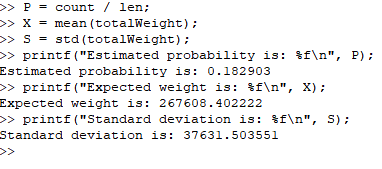
\includegraphics[scale=1.5]{screenshot.png} 




\end{document}